\section{问题重述与分析}

啤酒的风味由挥发性化合物、理化条件与酿造工艺共同决定：酯类与高级醇带来果香与醇厚感，酒花萜烯提供草本与柑橘调，硫化物、双乙酰、反式-2-壬烯醛等则构成缺陷。附件给出了 250 款商业啤酒的化合物测量与感官评分，要求完成三项任务：由化合物预测 0--6 分的感官画像；识别各感官维度的关键化合物并论证其稳定性与化学合理性；在给定风格下生成化合物谱，并把 Pils/Lager 迁移为 Tripel 而缺陷不恶化。

\subsection{三项任务要求的证据强度不同}

三项任务共享同一份数据与同一套验证框架，但它们要求的证据强度依次递增。第一问是\textbf{预测}：只要在留出酒样上误差可控、区间可信，结论即可成立。第二问是\textbf{解释}：模型选出的重要化合物必须同时满足统计稳定与化学可解释，而相关系数与回归系数都不构成因果。第三问是\textbf{决策}：生成谱与迁移候选要同时满足风格、感官与缺陷三类约束，模型内可行与真实可酿造之间还隔着制备与品评。

因此本文不为三问套用同一种评价：第一问报告按酒划分的留出误差与区间覆盖，第二问报告重采样频率与置换贡献，第三问报告冻结候选的三层复核与线性规划可行性证书。任何一问的好成绩都不自动支持另一问。

\subsection{技术路线}

图\ref{fig:roadmap}给出全文结构。数据层完成四件事：附件结构核查、化学尺度与缺失诊断、评分端点重建、评分卡到目标列的维度映射。任务层按三问展开，但共用同一批按酒分层的划分与同一套预处理规则。最底层是统一的验证约定：插补、截尾、标准化与调参只在训练折内估计，生成与迁移的候选先冻结再复核，失败与反直觉结果全部保留。

\begin{figure*}[t]
\centering
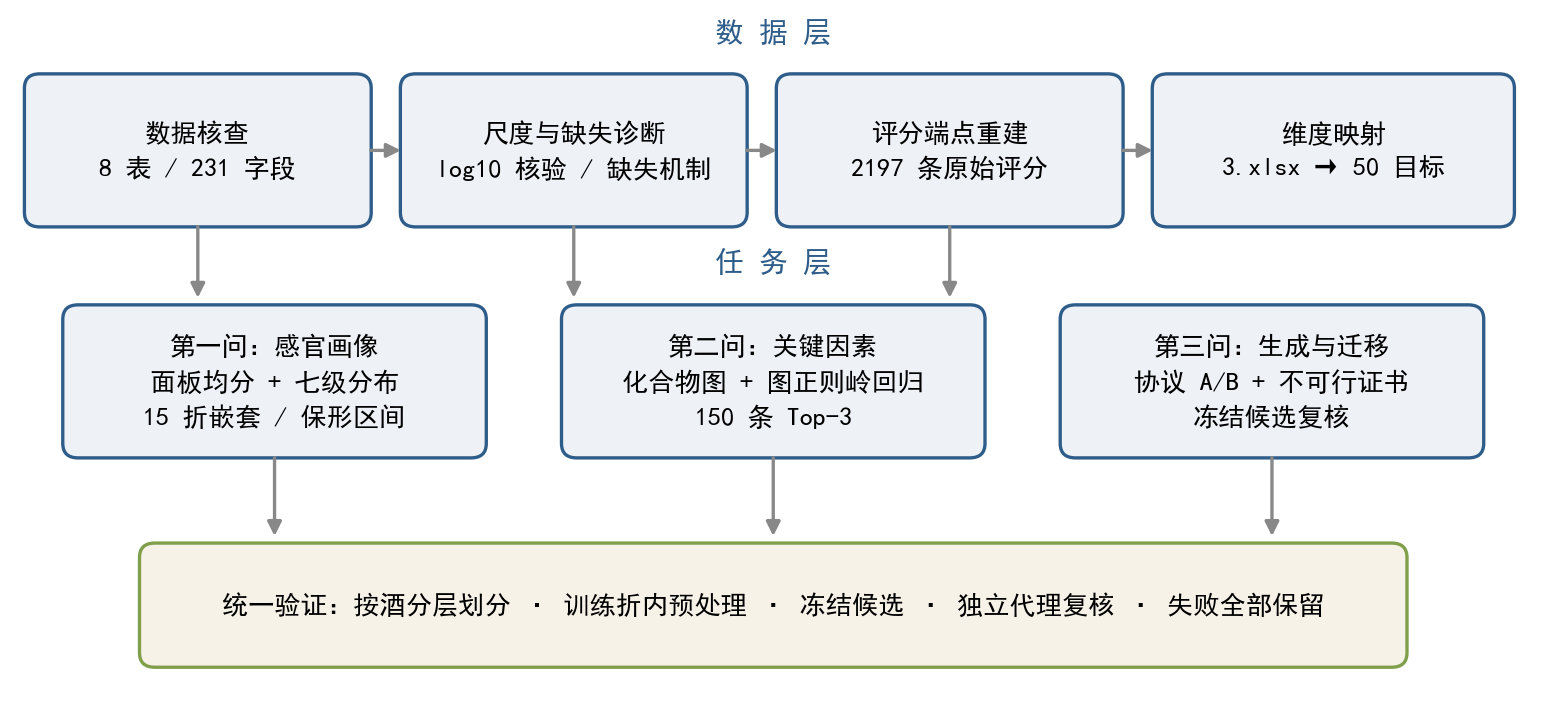
\includegraphics[width=0.98\textwidth]{figures/fig01_roadmap.png}
\caption{全文技术路线。数据层的四项核查共同决定任务层的输入口径；三问共用按酒分层划分与训练折内预处理，避免同一款酒同时出现在训练与验证中。}
\label{fig:roadmap}
\end{figure*}

\subsection{本文的交付物}

对应三问，本文给出四类可复核的结果：一是 250 款酒在 50 个感官目标上的面板均分与七级评分分布，以及据此得到的众数与中位数等级；二是 50 个目标各 3 个候选化合物、共 150 条因素记录，附重采样入选频率、置换贡献与化学依据；三是 Tripel、Kriek、Lambic 三种风格的生成谱及其感官画像；四是 Pils/Lager 到 Tripel 的迁移可行域，包括严格协议下的不可行证书与阈值协议下的可行记录数。

上述结果全部由可重跑的脚本产生，输入文件哈希、随机种子与运行配置随结果保存。第\ref{sec:data}节交代数据口径，第\ref{sec:q1}至\ref{sec:q3}节分别给出三问的模型与结果，第\ref{sec:eval}节讨论适用范围与推广。
